%%%%%%%%%%%%%%%%%%%%%%%%%%%%%%%%%%%%
% Slide options
%%%%%%%%%%%%%%%%%%%%%%%%%%%%%%%%%%%%

% Option 1: Slides with solutions

\documentclass[slidestop,compress,mathserif]{beamer}
\newcommand{\soln}[1]{\textit{#1}}
\newcommand{\solnGr}[1]{#1}

% Option 2: Handouts without solutions

%\documentclass[11pt,containsverbatim,handout]{beamer}
%\newcommand{\soln}[1]{ }
%\newcommand{\solnGr}[1]{ }

%%%%%%%%%%%%%%%%%%%%%%%%%%%%%%%%%%%%
% Style
%%%%%%%%%%%%%%%%%%%%%%%%%%%%%%%%%%%%

\usepackage{geometry}
\usepackage{graphicx}
\usepackage{amssymb}
%\usepackage{cancel}
\usepackage{epstopdf}
\usepackage{amsmath}  	% this permits text in eqnarray among other benefits
\usepackage{url}		% produces hyperlinks
\usepackage{hyperref}	% allows for color usage in tables
\usepackage[english]{babel}
\usepackage[latin1]{inputenc}
\usepackage{colortbl}	% allows for color usage in tables
\usepackage{multirow}	% allows for rows that span multiple rows in tables
\usepackage{color}		% this package has a variety of color options
\usepackage{pgf}
\usepackage{calc}
\usepackage{ulem}
\usepackage{multicol}
\usepackage{textcomp}
\usepackage{txfonts}
\usepackage{listings}
\usepackage{tikz}
\usepackage{array}
\usepackage{wasysym}
\usepackage{fancyvrb}

%%%%%%%%%%%%%%%%
% Remove navigation symbols
%%%%%%%%%%%%%%%%

\setbeamertemplate{navigation symbols}{}

%%%%%%%%%%%%%%%%
% Get rid of fancy enumerated list bullets
%%%%%%%%%%%%%%%%

\setbeamertemplate{enumerate items}[default]

%%%%%%%%%%%%%%%%
% Custom commands
%%%%%%%%%%%%%%%%

% degree
\newcommand{\degree}{\ensuremath{^\circ}}

% cite
\newcommand{\ct}[1]{
\vfill
{\tiny #1}}


% two col: two columns
\newenvironment{twocol}[4]{
\begin{columns}[c]
\column{#1\textwidth}
#3
\column{#2\textwidth}
#4
\end{columns}
}

% pr: left and right parentheses
\newcommand{\pr}[1]{
\left( #1 \right)
}

% solnMult: solutions for practice questions

\newcommand{\solnMult}[1]{
\item[] \vspace{-0.59cm}
\only<1>{\item #1}
\soln{\only<2->{\item #1}}
}

% cancel
\newcommand{\cancel}[1]{%
    \tikz[baseline=(tocancel.base)]{
        \node[inner sep=0pt,outer sep=0pt] (tocancel) {#1};
        \draw[red, line width=0.5mm] (tocancel.south west) -- (tocancel.north east);
    }%
}

% removepagenumbers
\newcommand{\removepagenumbers}{% 
  \setbeamertemplate{footline}{}
}



%%%%%%%%%%%%%%%%
% Graphics
%%%%%%%%%%%%%%%%

\DeclareGraphicsRule{.tif}{png}{.png}{`convert #1 `dirname #1`/`basename #1 .tif`.png}

%%%%%%%%%%%%%%%%%%%%%%%%%%%%%%%%%%%%
% Begin document
%%%%%%%%%%%%%%%%%%%%%%%%%%%%%%%%%%%%

\title[Chp 5.1: Small single sample (T distribution)]{Chp 5.1: Small single sample (T distribution)}

\begin{document}

\section{T distribution}

\begin{frame}
\frametitle{The $T$ distribution}
\begin{itemize}
\item With large samples, we can assume $\sigma \approx s$.
\pause
\item With small samples, there is usually uncertainty about $\sigma$. We have not accounted for this additional uncertainty until now.
\pause
\item With small $n$, sampling distributions (from approximately symmetric populations) follow the $T$ distribution, which is like the $Z$ distribution, but it has fatter tails.
\pause
\item As $n$ grows, the $T$ distribution approaches the $Z$ distribution.
\pause
\end{itemize}
\begin{center}
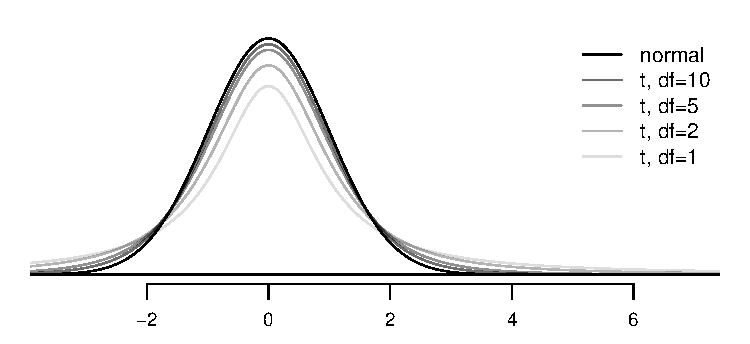
\includegraphics[scale=0.8]{figures/tDistConvergeToNormalDist/tDistConvergeToNormalDist.pdf}
\end{center}
\end{frame}


\section{t table}

\begin{frame}
\frametitle{Using the $t$ table}
\begin{itemize}
\item If $df=8$ and $P(T<t)=0.95$, what is $t$?\pause
\soln{$$t=1.86$$}\pause
\vfill
\item If $df=10$ and $P(|T|>t)=0.005$, what is $t$?\pause
\soln{$$t=3.58$$}\pause
\vfill
\item If $df=5$ what is $P(T>2.76)$?\pause
\soln{$$P(T>2.76) = 0.02$$}\pause
\vfill
\item If $df=5$ what is $P(T<-2.76)$?\pause
\soln{$$P(T<-2.76) = 0.02$$}\pause
\vfill
\end{itemize}
\end{frame}



\section{CI}

\begin{frame}
\frametitle{Example confidence interval of single sample with small $n$, unknown $\sigma$.}
A random sample of size $n=10$ was collected from a population which is believed to be approximately symmetric. The sample has a mean $\bar{x}=135.7$ and standard deviation $s=24.6$. Find the confidence interval with a confidence level $\gamma = 0.95$.
\pause

\begin{itemize}
\item The formulas:
\begin{align*}
SE &= \frac{s}{\sqrt{n}} \\
df &= n-1\\
P(|T|<t^{\star}) &= \gamma\\ 
CI &= \bar{x} \pm t^{\star} SE 
\end{align*}
\end{itemize}
\end{frame}


\begin{frame}
A random sample of size $n=10$ was collected from a population which is believed to be approximately symmetric. The sample has a mean $\bar{x}=135.7$ and standard deviation $s=24.6$. Find the confidence interval with a confidence level $\gamma = 0.95$.
\pause
\begin{itemize}
\item Calculate the standard error (same way as before).
\pause
$$SE = \frac{24.6}{\sqrt{10}} = 7.78 $$
\pause
\item Calculate the degrees of freedom.
\pause
$$df = 10-1 = 9 $$
\pause
\item Determine $t^\star$ such that $P(|T|<t^{\star}) = 0.95$. We use the $T$ table.
\pause
$$t^{\star} = 2.26 $$
\pause \vspace{-10pt}
\item Calculate the confidence interval.
\pause
$$CI = 135.7 \pm (2.26)(7.78) $$
$$CI = (118.1,\,153.3) $$
\end{itemize}
\end{frame}

\section{Practice CI}

\begin{frame}
\frametitle{Practice: confidence interval, single small sample, unknown $\sigma$}
A random sample of size $n=15$ was collected from a population which is believed to be approximately symmetric. The sample has a mean $\bar{x}=11.1$ and standard deviation $s=2.3$. Find the confidence interval with a confidence level $\gamma = 0.99$.
\pause
\solnGr{
$$SE = \frac{2.3}{\sqrt{15}} = 0.594 $$
\pause
$$df = 15-1 = 14 $$
\pause
Determine $t^\star$ such that $P(|T|<t^{\star}) = 0.99$. We use the $T$ table.
\pause
$$t^{\star} = 2.98 $$
\pause
$$CI = 11.1 \pm (2.98)(0.594) $$
\pause
$$CI = (9.33,\,12.87) $$
}
\end{frame}

\section{CI backwards}

\begin{frame}
\frametitle{Working backwards: confidence intervals}
A 90\% confidence interval for a population mean, \(\mu\), is given as
(43.84, 55.92). This confidence interval is based on a simple random
sample of 12 observations. Calculate the sample mean and standard
deviation. Assume that all conditions necessary for inference are
satisfied. Use the \(T\) distribution in any calculations.
\pause
\begin{itemize}
\item The formulas:
\begin{align*}
SE &= \frac{s}{\sqrt{n}} \\
df &= n-1\\
P(|T|<t^{\star}) &= \gamma\\ 
CI &= \bar{x} \pm t^{\star} SE 
\end{align*}
\end{itemize}
\end{frame}


\begin{frame}
The sample mean is the average of the bounds of the CI. \pause
\[\bar{x} = \frac{43.84 + 55.92}{2} = 49.88 \] \pause
The margin of error is half the difference between the bounds. It is also the distance from \(\bar{x}\) to either bound. \pause
\[ME = \frac{55.92-43.84}{2} = 55.92-49.88  = 6.04\] \pause
That margin of error is the product of \(t^{\star}\) and \(SE\). \pause We find the \(t^{\star}\) when \(P(|T|<t^{\star})=0.9\) and \(df=n-1=11\). \pause
\[t^{\star} = 1.8 \] 
\pause
We can calculate \(SE\).
\pause
 \[ME = t^{\star} SE \]
 
\pause
\[6.04 = (1.8) SE \]

\pause
\[SE = \frac{6.04}{1.8} = 3.3564258 \]

continued on next frame...
\end{frame}

\begin{frame}
\[SE = \frac{6.04}{1.8} = 3.3564258 \]

\pause
We can now calculate the sample standard deviation.
\[SE = \frac{s}{\sqrt{n}} \]

\pause
\[3.3564258 = \frac{s}{\sqrt{12}} \]

\pause
\[s = (3.356)\sqrt{12} = 11.627 \]

\pause
Thus, the sample mean is 49.88 and the sample standard deviation is
11.63.
\end{frame}


\section{Practice CI backwards}

\begin{frame}
\frametitle{Practice: working backwards with confidence intervals}
A 95\% confidence interval for a population mean, \(\mu\), is given as
(88.09, 109.15). This confidence interval is based on a simple random
sample of 9 observations. Calculate the sample mean and standard
deviation. Assume that all conditions necessary for inference are
satisfied. Use the \(T\) distribution in any calculations.
\pause
\soln{
$$\bar{x} = \frac{88.09 + 109.15}{2} = 98.62 $$
\pause
$$ME = \frac{109.15-88.09}{2} = 10.53 $$
\pause
$$df=8 $$
\pause \vspace{-5pt}
$$t^{\star} = 2.31 $$
\pause \vspace{-5pt}
$$SE = \frac{10.53}{2.31} = 4.56 $$
\pause \vspace{-5pt}
$$s = (4.56)\sqrt{9} = 13.68 $$
 }
\end{frame}



\section{Hypothesis testing with single small sample}

\begin{frame}
\frametitle{Hypothesis testing with single small sample}
You will perform a single-sample \(t\) test of the null hypothesis
claiming \(\mu=22\). Before collecting the sample, you decide to use a
two-tail test with a significance level \(\alpha = 0.05\). The sample
has the following attributes: \[\begin{aligned}
n &=& 11 \\
\bar{x} &=& 15.49 \\
s &=& 8.03
\end{aligned}\] What is your conclusion?

\pause 
We state the hypotheses:\pause \[H_0:~~\mu = 22 \] \[H_A:~~\mu \ne 22 \] 
\pause
We estimate the standard error (same way as with \(z\) testing). \pause
\[SE = \frac{s}{\sqrt{n}} =  \frac{8.03}{\sqrt{11}} = 2.421\]
continued on next slide...
\end{frame}

\begin{frame}
 We calculate the \(t\) score (same way as with \(z\) testing). \pause
\[t = \frac{15.49-22}{2.421} = -2.69 \] \pause 
For the $T$ table, we use the absolute value of $t$...
$$t = 2.69 $$
We determine the degrees of freedom. 
\[df = n-1 = 10 \] \pause We estimate the \(p\)-value from the \(T\)
table. \pause \[0.02 < p\text{-value} < 0.04 \] \pause We compare the \(p\)-value to \(\alpha\). \pause \[p\text{-value} < \alpha \] \pause We make our conclusion: we
reject the null.
\end{frame}


\section{Practice hypothesis testing}

\begin{frame}
\frametitle{Practice:}
You will perform a single-sample \(t\) test of the null hypothesis
claiming \(\mu=140\). Before collecting the sample, you decide to use a
two-tail test with a significance level \(\alpha = 0.1\). The sample has
the following attributes: \[\begin{aligned}
n &=& 3 \\
\bar{x} &=& 193.06 \\
s &=& 52.22
\end{aligned}\] What is your conclusion?


\end{frame}

\solnGr{
\begin{frame}
\footnotesize
We state the hypotheses: \pause \[H_0:~~\mu = 140 \] \[H_A:~~\mu \ne 140 \] \pause We
estimate the standard error (same way as with \(z\) testing).\pause 
\[SE = \frac{s}{\sqrt{n}} =  \frac{52.22}{\sqrt{3}} = 30.149\] \pause We
calculate the \(t\) score (same way as with \(z\) testing).\pause 
\[t = \frac{193.06-140}{30.149} = 1.76 \] \pause We determine the degrees of
freedom. \pause \[df = n-1 = 2 \] \pause  We estimate the \(p\)-value from the \(T\)
table. \pause  \[0.2 < p\text{-value} < 0.5 \] \pause  We compare the \(p\)-value to
\(\alpha\). \pause  \[p\text{-value} > \alpha \] \pause  We make our conclusion: \pause  we
retain the null.
\end{frame}
}

\end{document}
